\documentclass[12pt,a4paper]{article}
\usepackage{fontspec}
\usepackage{polyglossia}
\setdefaultlanguage{english}
\setotherlanguage{thai}
\setmainfont{Sarabun}
\setsansfont{Sarabun}
\newfontfamily\thaifont[Script=Thai]{Sarabun}
\setmonofont{Menlo}[Scale=MatchLowercase]
\usepackage[top=2.4cm,bottom=2.35cm,left=2.5cm,right=2.5cm,headheight=16pt]{geometry}
\usepackage{graphicx,longtable,array,booktabs,xcolor,colortbl,float,enumitem,needspace,caption}
\usepackage{amsmath}
\usepackage{fancyhdr,titlesec,listings,xurl,hyperref,pdflscape}
\definecolor{KeyGreen}{HTML}{087A46}
\definecolor{SoftGreen}{HTML}{EAF4EE}
\definecolor{CodeTint}{HTML}{FFFFFF}
\definecolor{RuleGray}{HTML}{C8C8C8}
\definecolor{CaptionBlue}{HTML}{0000EE}
\hypersetup{unicode=true,colorlinks=true,linkcolor=black,urlcolor=KeyGreen,pdftitle={CPE333 Mini-Project 2: Virtual Memory},hypertexnames=false}
\urlstyle{same}
\setlength{\emergencystretch}{2em}
\widowpenalty=10000
\clubpenalty=10000
\setlength{\parindent}{0pt}
\setlength{\parskip}{5.5pt}
\setlength{\tabcolsep}{5pt}
\renewcommand{\arraystretch}{1.25}
\renewcommand{\thesection}{}
\renewcommand{\thesubsection}{}
\renewcommand{\thesubsubsection}{\arabic{subsection}.\arabic{subsubsection}}
\setcounter{tocdepth}{2}
\titleformat{\section}{\color{black}\fontsize{16}{19.2}\selectfont\bfseries}{}{0pt}{}
\titleformat{\subsection}{\color{black}\fontsize{14}{17.5}\selectfont\bfseries}{}{0pt}{}
\titleformat{\subsubsection}{\color{black}\fontsize{12}{15.6}\selectfont\bfseries}{}{0pt}{}
\titlespacing*{\section}{0pt}{15pt}{6pt}
\titlespacing*{\subsection}{0pt}{10pt}{3pt}
\titlespacing*{\subsubsection}{0pt}{8pt}{3pt}
\DeclareCaptionFont{capfont}{\color{CaptionBlue}\itshape\fontsize{12}{15.5}\selectfont}
\captionsetup{font=capfont,labelfont=bf,skip=7pt}
\newcommand{\keyterm}[1]{\textcolor{KeyGreen}{\textbf{#1}}}
\newcommand{\code}[1]{{\fontspec{Menlo}\fontsize{9.5}{12}\selectfont\color{KeyGreen!85!black}\let\codeunderscore\_\def\_{\codeunderscore\allowbreak}#1}}
\lstset{basicstyle=\fontspec{Menlo}\fontsize{9.5}{12}\selectfont,columns=fullflexible,keepspaces=true,breaklines=true,showstringspaces=false,backgroundcolor=\color{CodeTint},frame=single,rulecolor=\color{black},framesep=5pt,aboveskip=7pt,belowskip=8pt,xleftmargin=.1cm,tabsize=4,keywordstyle=\color{blue}\bfseries,commentstyle=\color{gray},stringstyle=\color{magenta}}
\pagestyle{fancy}\fancyhf{}
\fancyfoot[C]{\fontsize{10}{12}\selectfont\thepage}
\renewcommand{\headrulewidth}{0pt}
\AtBeginDocument{\fontsize{12}{15.6}\selectfont}
\begin{document}
\newgeometry{top=1.7cm,bottom=2.35cm,left=2.5cm,right=2.5cm,headheight=16pt}
\begin{titlepage}\thispagestyle{empty}\centering

\includegraphics[width=3.5cm]{assets/KMUTT_Logo.png}\par\vspace{.10cm}
{\fontsize{14.5}{17.5}\selectfont MINI-PROJECT 2\par}
\vspace{.04cm}
{\fontsize{13.5}{16.5}\selectfont Virtual Memory\par}
\vspace{2.20cm}
{\fontsize{12.5}{15.5}\selectfont Prepared by\par}
\vspace{.10cm}
{\fontsize{12}{15}\selectfont Group: }{\thaifont\fontsize{12}{15}\selectfont มูลนิธิทนายตั้ม ช่วยสู้\par}
\vspace{1.00cm}
{\fontsize{12}{15}\selectfont
\renewcommand{\arraystretch}{1.70}
\begin{tabular}{>{\raggedright\arraybackslash}p{9.8cm}>{\raggedleft\arraybackslash}p{3.1cm}}
Guntee Doungmanee & 67070501003\\
Drarun Yookphan & 67070501016\\
Natthawat Primsirikunawut & 67070501027\\
Rattathamnoon Buranapattana & 67070501037\\
Wisit Suwannao & 67070501042\\
Supawit Marayat & 67070501045\\
Polwarit Watthanahemmarat & 67070501067\\
\end{tabular}\par}
\vspace{1.40cm}
{\fontsize{12}{15}\selectfont Submitted to\par}
\vspace{.20cm}
{\fontsize{12}{15}\selectfont Asst. Prof. Rajchawit Sarochawikasit\par}
\vspace{.65cm}
{\fontsize{12}{26.8}\selectfont
This report is part of CPE333 Operating Systems\\
Department of Computer Engineering, Faculty of Engineering\\
King Mongkut's University of Technology Thonburi\\
Semester 1, Academic Year 2026\par}
\end{titlepage}
\restoregeometry
\clearpage\pagenumbering{roman}
\tableofcontents
\clearpage\pagenumbering{arabic}

\Needspace{6\baselineskip}
\section{Problem 1: Project scope and design}

The project is a Linux tool for inspecting a process's \keyterm{memory regions}, \keyterm{virtual address space}, and \keyterm{minor and major page faults}. It combines the \code{pfcount} kernel module, the \code{pfstat} command-line program, and the \code{faultgen} workload generator. We tested the merged PR \#11 source on Ubuntu 24.04.5 with Linux 6.8.0-142-generic on ARM64. The build, demo, regression suite, and experiments E1 to E8 all completed in that environment.

These measurements describe different things. A process can reserve a large virtual range before its pages become resident, and file cache, readahead, fault-around, and Transparent Huge Pages (THP) can all change the recorded fault counts. The results describe the tested kernel configuration; they do not establish compatibility with other kernels or measure probe overhead.

\begin{table}[H]\centering
{\fontsize{12}{15.6}\selectfont\arrayrulecolor{RuleGray}
\caption{Project requirements and how we checked them}
\begin{tabular}{|>{\raggedright\arraybackslash}p{3.5cm}|>{\raggedright\arraybackslash}p{5.8cm}|>{\raggedright\arraybackslash}p{5.2cm}|}
\hline
\rowcolor{SoftGreen} \textbf{Requirement} & \textbf{Implementation} & \textbf{Check} \\ \hline
Select a process & \code{pfstat PID} writes the target PID to \code{/proc/pfcount/target} & Read the report for a stable process \\ \hline
Count memory regions & Walk the process's VMAs & Compare with \code{/proc/PID/maps} \\ \hline
Measure virtual address space & Sum \code{vm\_end - vm\_start} for every VMA & Compare with maps, \code{mm->total\_vm}, and VmSize \\ \hline
Count minor and major faults & Read lifetime counters and count live faults with a kretprobe & Compare with kernel counters using the same process scope \\ \hline
Explain Virtual Memory behavior & Relate VMAs, demand paging, cache, and THP to E1 to E8 & Analyze the measured results in Problem 2, Step 2 \\ \hline
\end{tabular}}
\end{table}

The required output is the four process-level measurements listed above. Watch mode, run mode, descendant tracking, RSS reporting, and exit-time snapshots are additional features. We tested the tool in one Linux VM with one kernel configuration, described in Problem 2, Step 1.

\Needspace{6\baselineskip}
\subsection{Step 1: Virtual memory and page faults}

\subsubsection{Virtual address space and VMAs}

A process uses a \keyterm{virtual address space} that Linux describes through \code{struct mm\_struct}. The kernel divides it into \keyterm{Virtual Memory Areas (VMAs)}. Each VMA is a contiguous address range with common permissions and backing information. Its start and end addresses are \code{vm\_start} and \code{vm\_end}, so its size is their difference [3].

A VMA may contain many pages. The number of VMAs therefore is not the number of pages or the amount of resident memory. Summing the VMA sizes gives the mapped virtual address space. Comparing this value with RSS shows how much address space is mapped and how much memory is resident. Experiment E7 uses both measurements to illustrate demand paging.

\subsubsection{Page faults and fault classification}

With \keyterm{demand paging}, Linux prepares a page when a process first accesses it. A \keyterm{minor fault} can be handled without storage I/O. A \keyterm{major fault} requires I/O to obtain the page [4]. These counters record kernel fault events. They do not count load/store instructions or device I/O requests.

The module reads the return value from \code{handle\_mm\_fault()} and applies the classification rules used by \code{mm\_account\_fault()} in the tested kernel. A \code{VM\_FAULT\_RETRY} result is not counted until the final attempt completes. A \code{VM\_FAULT\_ERROR} result is recorded as a failed fault. A successful result is major when \code{VM\_FAULT\_MAJOR} is set or the original flags contain \code{FAULT\_FLAG\_TRIED}; otherwise, it is minor [2, 5].

\Needspace{10\baselineskip}
\begin{lstlisting}[language=C]
if (ret & VM_FAULT_RETRY)
    /* wait for the final attempt */;
else if (ret & VM_FAULT_ERROR)
    /* record a failed fault */;
else if ((ret & VM_FAULT_MAJOR) || (flags & FAULT_FLAG_TRIED))
    /* count a major fault */;
else
    /* count a minor fault */;
\end{lstlisting}

The assignment suggests the \code{exceptions:page\_fault\_user} tracepoint. That tracepoint belongs to the x86 page-fault path, while our test VM is ARM64. It also fires before the kernel has finished handling the fault, so it does not directly provide the information needed to distinguish minor from major faults [2, 5]. We instead use a kretprobe on \code{handle\_mm\_fault()} and classify the completed result. This choice matches the Linux 6.8 accounting rules used in the test environment. We did not measure the probe's performance overhead systematically.

\Needspace{8\baselineskip}
\subsubsection{Page cache, readahead, and huge pages}

A file-backed mapping can use the \keyterm{page cache} without a new device read. We separated cold-cache and warm-cache cases and used \code{MADV\_RANDOM} in selected tests to reduce readahead. On the tested kernel, disabling readahead did not disable fault-around. Linux could still map nearby pages that were already in the cache.

\keyterm{Transparent Huge Pages (THP)} can also change fault counts. The \code{faultgen} program requests THP with \code{MADV\_HUGEPAGE} and ordinary pages with \code{MADV\_NOHUGEPAGE}. These calls advise the kernel but do not guarantee that every mapping receives a huge page [6]. The fault counts therefore describe the workload; on their own, they do not prove that every requested mapping used THP.

\Needspace{6\baselineskip}
\subsection{Step 2: How the tool works}

\begin{figure}[H]\centering
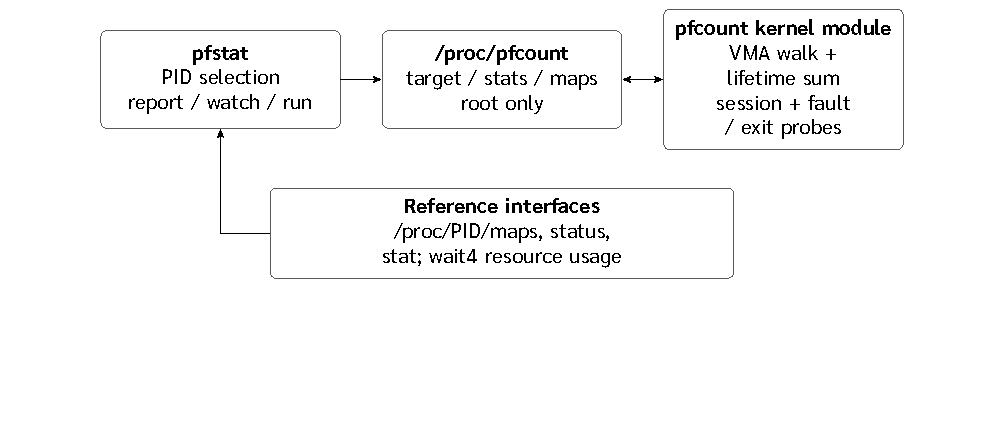
\includegraphics[width=\linewidth]{assets/architecture.pdf}
\caption{User-space tools, kernel data sources, and comparison interfaces}\end{figure}

\subsubsection{Counting regions and virtual address space}

When a user selects a PID, \code{pfstat} writes it to \code{/proc/pfcount/target} and reads the module's stats and maps interfaces. The module obtains a reference to the process address space with \code{get\_task\_mm()}, takes \code{mmap\_read\_lock\_killable()}, and walks the VMAs with \code{VMA\_ITERATOR} and \code{for\_each\_vma}. It then releases the lock and the address-space reference with \code{mmput()} [2, 3].

For each VMA, the module increments the region count and adds \code{vm\_end - vm\_start} to the virtual size. It also groups mappings as file-backed, anonymous, heap, stack, or special mappings. Those groups help explain the output; they do not change the definition of a region. The module's total is checked against the address ranges in \code{/proc/PID/maps}, \code{mm->total\_vm}, and VmSize.

\Needspace{13\baselineskip}
\begin{lstlisting}[language=C]
mm = get_task_mm(task);
mmap_read_lock_killable(mm);
VMA_ITERATOR(vmi, mm, 0);
for_each_vma(vmi, vma) {
    regions++;
    vsize += vma->vm_end - vma->vm_start;
}
mmap_read_unlock(mm);
mmput(mm);
\end{lstlisting}

This snippet shows the main sequence. The implementation also handles a missing task, a task without an address space, and an interrupted lock acquisition.

\subsubsection{Lifetime and live fault counters}

Lifetime counters combine \code{min\_flt} and \code{maj\_flt} values from live threads with totals transferred to \code{signal\_struct} when threads exit. The reviewed source uses \code{sig->stats\_lock} and a sequence/retry pattern like \code{/proc/PID/stat}. This avoids counting a thread twice or reading it while its totals are being transferred [2, 7]. These counters cover the thread group from process start.

Live counters start when the user selects a target. On entry to the \code{handle\_mm\_fault()} kretprobe, the module checks whether the faulting process is in scope and saves the flags and backing type for that invocation. On return, it uses the completed result to update minor, major, anonymous, file-backed, or error counters. Keeping entry data with its invocation prevents the module from classifying a fault from a CPU error code before the kernel has handled it [2, 5, 8].

\subsubsection{Target sessions and process identity}

Each target selection creates a new \code{pf\_session} with a PID reference, start time, and its own counters. The probe entry handler holds a reference to the session that accepted a fault until the return handler finishes. A fault that began under an earlier target therefore cannot increment the new target's counters. RCU publication and reference counting let an in-flight handler finish safely while the target changes.

The module compares the thread-group \code{struct pid}, not only the numeric TGID. The kernel may reuse a PID after reaping the original process. Holding a reference to the PID object keeps the module from treating a new process with the same number as the original target. Problem 2, Step 3 checks this behavior with the PID-reuse regression.

\subsubsection{Exit snapshots and permissions}

For a short-lived process that exits before the user reads its stats, the module captures the region count, virtual size, and peak size through a kprobe on \code{acct\_collect(exitcode, group\_dead)}. The kernel calls this function after \code{atomic\_dec\_and\_test()} identifies the last thread and before \code{exit\_mm()}, while the address-space counters are still available. The probe uses \code{group\_dead} rather than guessing that a thread is last from \code{signal->live == 1} at the start of \code{do\_exit()} [2, 9].

The module sets permissions to 0600 for \code{/proc/pfcount/target} and 0400 for \code{stats} and \code{maps}. The interface can inspect the address space of a PID that the caller could not otherwise read, so the files are restricted to root. Our tests invoked the tool with \code{sudo}.

\subsubsection{Command-line modes}

\begin{table}[H]\centering
{\fontsize{12}{15.6}\selectfont\arrayrulecolor{RuleGray}
\caption{Main pfstat modes}
\begin{tabular}{|>{\raggedright\arraybackslash}p{6.4cm}|>{\raggedright\arraybackslash}p{8.2cm}|}
\hline
\rowcolor{SoftGreen} \textbf{Command} & \textbf{Behavior} \\ \hline
\code{sudo tools/pfstat PID} & Print one summary and compare it with procfs \\ \hline
\code{sudo tools/pfstat PID --maps} & Include the process's VMA list \\ \hline
\code{sudo tools/pfstat PID -w 0.5} & Sample repeatedly and calculate rates using elapsed time \\ \hline
\code{sudo tools/pfstat -- CMD} & Run a command and count faults from before exec until exit \\ \hline
\code{sudo tools/pfstat -f -- CMD} & Include descendants that remain within the tracked ancestry \\ \hline
\end{tabular}}
\end{table}

In run mode, the parent stops the child with SIGSTOP, selects it as the target, reads the lifetime baseline, and then allows it to exec the requested command. The program subtracts that baseline before comparing its live counters with \code{wait4()}. The child drops back to the invoking user's privileges before exec. After fork, the program restores the inherited SIGCHLD disposition in the child and uses a cleanup path to reset the target and follow state if execution or waiting fails. The post-merge test also covers a parent that inherited \code{SIGCHLD=SIG\_IGN}.

The terminal report below is a separate example for the current shell. It shows the VMA total, virtual size, fault counters, and mapping groups in one view; the E1 measurements that follow use the recorded \code{sleep} and PID 1 runs.

\begin{figure}[H]\centering
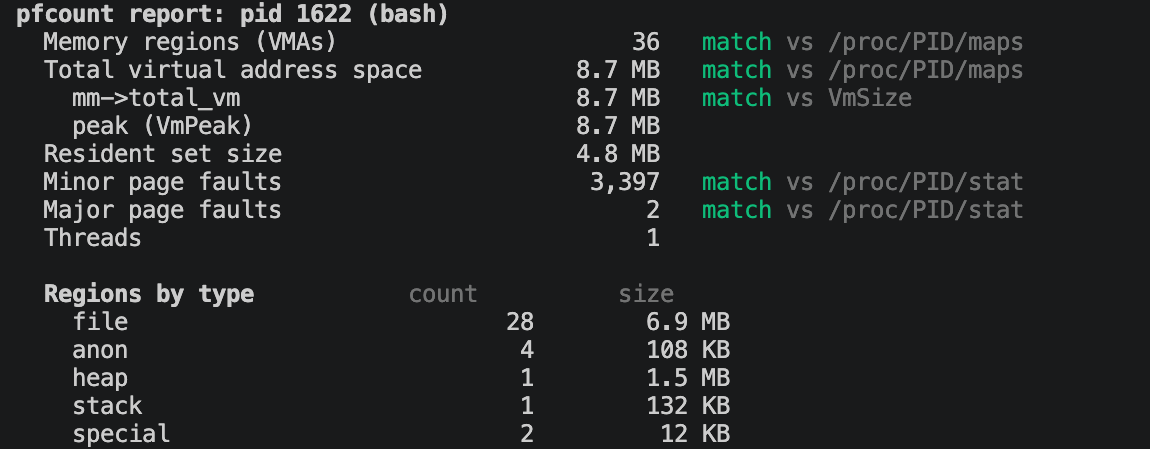
\includegraphics[width=\linewidth]{evidence/post-merge-5fbcb76/terminal/05-pfstat-report-terminal.png}
\caption{Example \texttt{pfstat} report for the shell, including procfs comparisons and VMA groups.}
\end{figure}

\Needspace{5\baselineskip}
In this shell example, the report finds 36 VMAs and 8.7 MB of virtual space. Both values match the mapping ranges in the process's \code{maps} file. \code{mm->total\_vm} matches VmSize, and 3,397 minor and 2 major faults match the corresponding \code{stat} counters. The final rows group the VMAs by backing type.

\Needspace{6\baselineskip}
\Needspace{12\baselineskip}
\section{Problem 2: Experimental method and results}

\subsection{Step 1: Test environment and method}

\begin{table}[H]\centering
{\fontsize{12}{15.6}\selectfont\arrayrulecolor{RuleGray}
\caption{Post-merge test environment}
\begin{tabular}{|>{\raggedright\arraybackslash}p{4.2cm}|>{\raggedright\arraybackslash}p{10.4cm}|}
\hline
\rowcolor{SoftGreen} \textbf{Item} & \textbf{Value} \\ \hline
Host and virtual machine & macOS host; Lima VM with 4 reported vCPUs and 3,905 MB guest memory \\ \hline
Guest and kernel & Ubuntu 24.04.5 LTS; Linux 6.8.0-142-generic; aarch64 \\ \hline
Compiler & GCC 13.3.0 \\ \hline
Page size and THP & 4,096 bytes; THP mode set to \code{madvise} \\ \hline
Fault-around and readahead & 65,536 bytes and 128 KiB, respectively \\ \hline
Kernel options & \code{CONFIG\_KPROBES=y}, \code{CONFIG\_KRETPROBES=y}, \code{CONFIG\_BSD\_PROCESS\_ACCT=y} \\ \hline
Source revision & PR \#11 merge commit \code{5fbcb767} \\ \hline
\end{tabular}}
\end{table}

The saved environment record identifies the guest kernel, required kernel options, and exact merge commit used for the post-merge measurements. The capture below isolates the three required kernel options so they remain readable at print size; the kernel version and architecture are recorded in the terminal output above.

\begin{lstlisting}
commit: 5fbcb7679298f36e2bae8b7cd3dbe6bf6a609800
Linux lima-cpe333 6.8.0-142-generic #142-Ubuntu SMP PREEMPT_DYNAMIC Wed Sep 2 14:30:29 UTC 2026 aarch64 aarch64 aarch64 GNU/Linux
CONFIG_BSD_PROCESS_ACCT=y
CONFIG_KPROBES=y
CONFIG_KRETPROBES=y
\end{lstlisting}

\begin{figure}[H]\centering
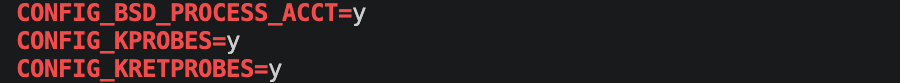
\includegraphics[width=\linewidth]{evidence/post-merge-5fbcb76/terminal/01-kernel-options-terminal.png}
\caption{Terminal output confirming the kernel options required by the module.}
\end{figure}

We kept raw outputs and environment details in the \code{evidence/} directory so the post-merge measurements remain separate from earlier PR tests. The program labels sizes as MB and KB but uses a base of 1,024. This report uses MiB and KiB when stating exact sizes; for example, \code{anon:64} means 64 MiB.

\Needspace{15\baselineskip}
\subsubsection{Build and load}

Inside Ubuntu, \code{vm.sh} prepared the Lima VM and installed build tools and headers matching \code{uname -r}. The build and load command, \code{make clean \&\& make all \&\& make load}, completed and created \code{/proc/pfcount/maps}, \code{/proc/pfcount/stats}, and \code{/proc/pfcount/target}.

The build reported a compiler-name mismatch despite GCC 13.3.0, shared-folder clock skew, and skipped BTF because \code{vmlinux} was unavailable. Kbuild still completed and the module loaded. Other kernels and architectures were not tested.

\begin{lstlisting}
./vm.sh setup
./vm.sh make clean
./vm.sh make all
./vm.sh make load
./vm.sh make demo
./vm.sh make experiments
./vm.sh run sudo sh tests/regress.sh
./vm.sh make unload
./vm.sh make clean
\end{lstlisting}

The saved build/load log records the object compilation, module link, and proc entries. Workspace-specific path prefixes are omitted here.

\begin{lstlisting}
make -C module
  CC [M] pfcount.o
  MODPOST Module.symvers
  LD [M] pfcount.ko
  BTF [M] pfcount.ko
Test binaries compiled: faultgen, threadexit, threadchurn, uffdblock
/proc/pfcount/: maps, stats, target
\end{lstlisting}

\begin{figure}[H]\centering
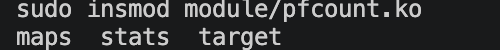
\includegraphics[width=.92\linewidth]{evidence/post-merge-5fbcb76/terminal/02-build-load-terminal.png}
\caption{Terminal output confirming that the loaded module exposes its proc interfaces.}
\end{figure}

\Needspace{40\baselineskip}
\subsubsection{End-to-end demo}

The demo command was \code{sudo tools/pfstat -w 0.5 -- tests/faultgen} with the workload phases \code{sleep:1 anon:64 sleep:1 file:/tmp/pfcount-big.bin sleep:1 free sleep:1}. The complete interval samples, rates, workload checkpoints, and exit summary below come from the saved terminal output in \code{evidence/post-merge-5fbcb76/02-demo-terminal-capture.txt}. The \code{faultgen} checkpoints are cumulative from process start, while \code{pfstat} subtracts the baseline recorded before \code{exec}; in this run that excludes 472 earlier minor faults. The resulting 16,782 minor and 4,097 major faults match the baseline-adjusted \code{getrusage()} comparison.

\begin{lstlisting}[basicstyle=\fontspec{Menlo}\fontsize{9}{10.8}\selectfont]
[faultgen 1935] start                        minflt=601 majflt=1
[faultgen 1935] anon 64 MB (16384 pages)     minflt=16998 majflt=1
[faultgen 1935] file 32768 KB (8192 pages)   minflt=17254 majflt=4097
[faultgen 1935] free                         minflt=17254 majflt=4097
[faultgen 1935] done                         minflt=17254 majflt=4097
    time  regions       vsize         rss      minflt    majflt     min/s    maj/s
     0.0        1        4 KB        0 KB         564         0         0        0
     0.5       16      2.2 MB      1.4 MB         614         1        99        2
     1.0       17     66.2 MB      9.1 MB       2,593         1     3,915        0
     1.5       17     66.2 MB     65.4 MB      16,998         1    28,668        0
     2.0       17     66.2 MB     65.4 MB      16,998         1         0        0
     2.5       18     98.2 MB     97.2 MB      17,254     4,097       511    8,173
     3.0       18     98.2 MB     97.2 MB      17,254     4,097         0        0
     3.5       16      2.2 MB      1.4 MB      17,254     4,097         0        0
     4.0       16      2.2 MB      1.4 MB      17,254     4,097         0        0

pfcount run: tests/faultgen ... (pid 1935, 4.54s, exit 0)
  Memory regions at exit                    16
  Virtual address space at exit         2.2 MB
  Peak virtual address space           98.2 MB
  Minor page faults                     16,782   match vs getrusage()
  Major page faults                      4,097   match vs getrusage()
    on anonymous memory                 16,454
    on file-backed memory                4,425
  fault scope: process only
\end{lstlisting}

\begin{figure}[H]\centering
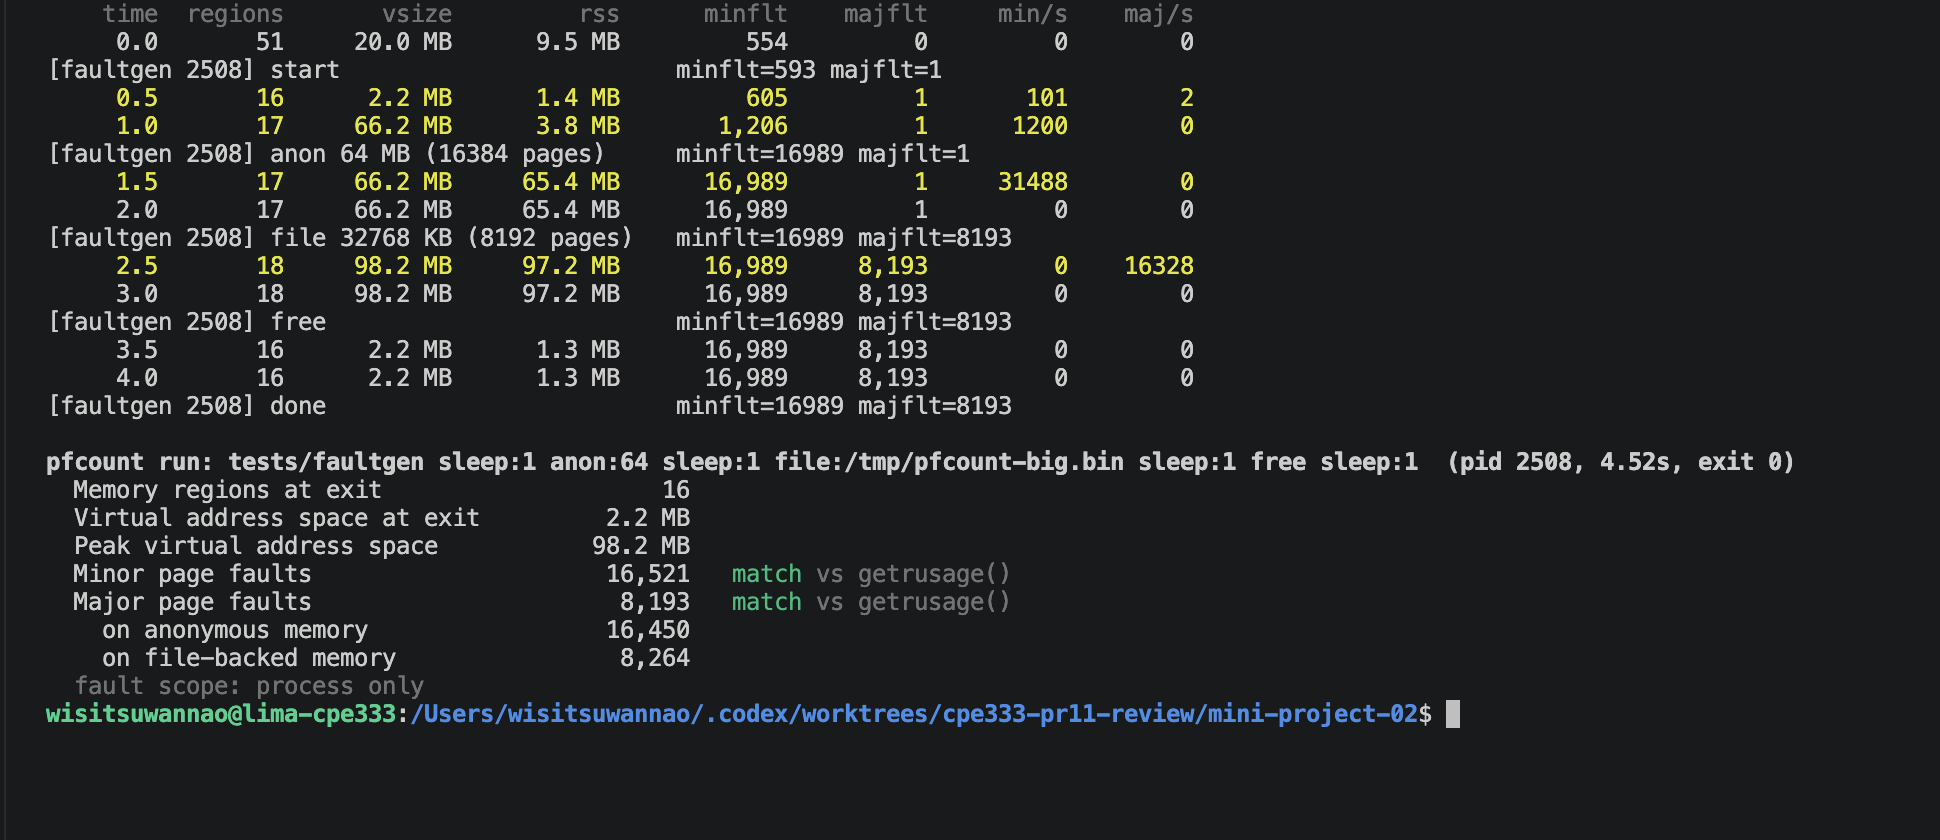
\includegraphics[width=.95\linewidth]{evidence/post-merge-5fbcb76/terminal/03-demo-terminal.png}
\caption{Terminal capture from a separate demo run. Fault totals vary with cache state; the latest transcript above supplies the values used in the analysis.}
\end{figure}

\subsubsection{How we checked the results}

We compared region counts and address-space sizes using a process that remained stable while the module and procfs were read. In run mode, we compared the final live counters with the child usage returned after exit, after subtracting the lifetime baseline. Agreement between these interfaces supports the observed behavior in the tested cases; both still rely on counters maintained by the same Linux kernel.

E1 compared the report with procfs. E2 to E6 varied anonymous mappings, file cache, readahead, and THP. E7 recorded virtual size and RSS over time and then unmapped the regions. E8 compared ordinary programs with and without descendant tracking. The post-merge regression suite covered retargeting, PID reuse, simultaneous thread exit, lifetime counter reads, module unload during a blocked fault, and cleanup after inherited SIGCHLD settings. Permission checks and interval parameters were present in earlier PR evidence; the post-merge suite summarized here did not rerun the non-root permission case.

\begin{figure}[H]\centering
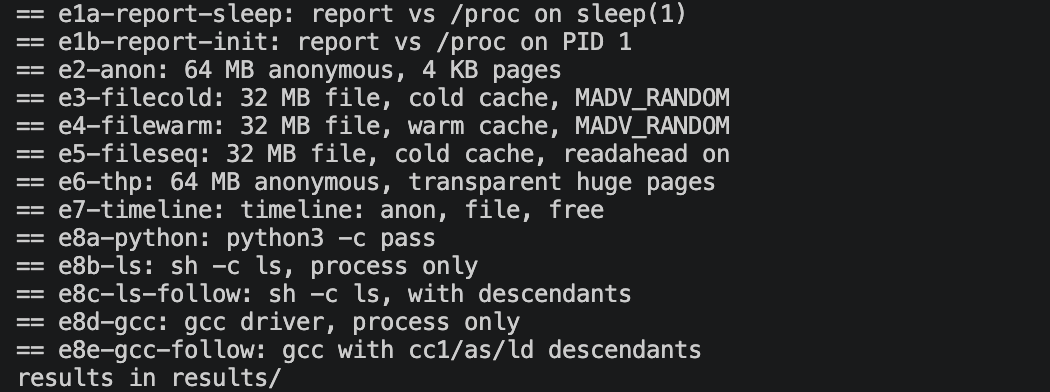
\includegraphics[width=.95\linewidth]{evidence/post-merge-5fbcb76/terminal/06-experiments-terminal.png}
\caption{Terminal summary of the E1 to E8 cases run by the experiment script. Numeric results appear in the following tables and discussion.}
\end{figure}

\Needspace{12\baselineskip}
\subsection{Step 2: Results}

\subsubsection{E1: comparison with procfs}

\begin{table}[H]\centering
{\fontsize{12}{15.6}\selectfont\arrayrulecolor{RuleGray}
\caption{E1 results from merge commit 5fbcb767}
\begin{tabular}{|>{\raggedright\arraybackslash}p{3.0cm}|>{\raggedright\arraybackslash}p{2.0cm}|>{\raggedright\arraybackslash}p{3.0cm}|>{\raggedright\arraybackslash}p{3.0cm}|>{\raggedright\arraybackslash}p{2.2cm}|}
\hline
\rowcolor{SoftGreen} \textbf{Target} & \textbf{Regions} & \textbf{Virtual size} & \textbf{Minor faults} & \textbf{Major faults} \\ \hline
\code{sleep} & 30 & 5.6 MB & 106 & 0 \\ \hline
PID 1, \code{systemd} & 113 & 21.9 MB & 12,986 & 94 \\ \hline
\end{tabular}}
\end{table}

The saved E1 logs also contain the mapping breakdown. These condensed output records omit region addresses and keep the cross-checks and VMA groups together:

\begin{lstlisting}
sleep (pid 10605): 30 VMAs, 5.6 MB; 106 minor, 0 major
  maps, VmSize, and /proc/PID/stat comparisons: match
  file 24/5.2 MB; anon 2/56 KB; heap 1/132 KB; stack 1/132 KB; special 2/12 KB
systemd (pid 1): 113 VMAs, 21.9 MB; peak 22.0 MB; RSS 12.1 MB
  12,986 minor, 94 major; maps, VmSize, and /proc/PID/stat comparisons: match
  file 98/18.5 MB; anon 11/356 KB; heap 1/2.9 MB; stack 1/132 KB; special 2/12 KB
\end{lstlisting}

For both targets, the region count and summed address ranges matched \code{maps}. The module's \code{mm->total\_vm} matched VmSize, and its lifetime fault counts matched \code{stat} in the recorded reads. PID 1 provided a system-process check under root. Its fault count changes with system activity, so these values describe the recorded run rather than a fixed property of PID 1.

\subsubsection{E2 to E6: mapping type and memory settings}

\begin{table}[H]\centering
{\fontsize{12}{15.6}\selectfont\arrayrulecolor{RuleGray}
\caption{Live fault counts compared with wait4() after baseline subtraction}
\begin{tabular}{|>{\raggedright\arraybackslash}p{.9cm}|>{\raggedright\arraybackslash}p{5.4cm}|>{\raggedright\arraybackslash}p{2.3cm}|>{\raggedright\arraybackslash}p{2.3cm}|>{\raggedright\arraybackslash}p{3.1cm}|}
\hline
\rowcolor{SoftGreen} \textbf{Test} & \textbf{Workload} & \textbf{Minor} & \textbf{Major} & \textbf{Comparison} \\ \hline
E2 & Anonymous mapping, 64 MiB & 16,538 & 1 & Match \\ \hline
E3 & Cold file, 32 MiB, RANDOM & 143 & 8,193 & Match \\ \hline
E4 & Warm file, 32 MiB, RANDOM & 652 & 1 & Match \\ \hline
E5 & Cold file, 32 MiB, readahead & 655 & 2 & Match \\ \hline
E6 & Anonymous mapping, 64 MiB, THP request & 188 & 1 & Match \\ \hline
\end{tabular}}
\end{table}

E2 wrote once to each ordinary page in a 64 MiB anonymous mapping. At a 4 KiB page size, the mapping contains 16,384 pages. The 16,538 minor faults also include process startup activity while monitoring was active, so the process-wide total is not expected to equal the number of intentional writes exactly.

E3 read a 32 MiB file, or 8,192 pages, after requesting that its data be dropped from the page cache. The program used \code{MADV\_RANDOM}. It recorded 8,193 major faults, including one that occurred before the file read. The increase during the read is consistent with 8,192 pages; major faults do not directly count device I/O requests.

E4 read a file already in cache. It produced mostly minor faults, and far fewer file faults than the 8,192 pages in the file. This result is consistent with fault-around mapping multiple nearby cached pages per fault. The configured \code{fault\_around\_bytes=65536} spans 16 ordinary pages. E5 enabled readahead for a cold file and recorded 2 major faults, compared with 8,193 in E3. Together, these runs show that fault counts depend on cache state, readahead, and fault-around, not only file size.

E6 requested THP for a 64 MiB anonymous mapping and recorded substantially fewer minor faults than E2. This is consistent with a fault mapping more memory at a time. If the kernel backs the whole region with 2 MiB huge pages, it would use about 32 such pages, but startup and other activity remain in the process-wide count. We did not collect \code{AnonHugePages} for every mapping, so the fault count alone does not confirm that all requested pages became huge pages.

The saved run summaries also show how the counts split between anonymous and file-backed memory. Each pair below matched the corresponding \code{getrusage()} result.

\begin{lstlisting}
E2 anon:64       minflt=16,538  majflt=1  anon=16,462  file-backed=77
E3 filecold      minflt=143     majflt=8,193  anon=71  file-backed=8,265
E4 filewarm      minflt=652     majflt=1  anon=68  file-backed=585
E5 fileseq       minflt=655     majflt=2  anon=72  file-backed=585
E6 thp:64        minflt=188     majflt=1  anon=112  file-backed=77
fault scope: process only
\end{lstlisting}

\subsubsection{E7: virtual size and RSS over time}

\begin{figure}[H]\centering
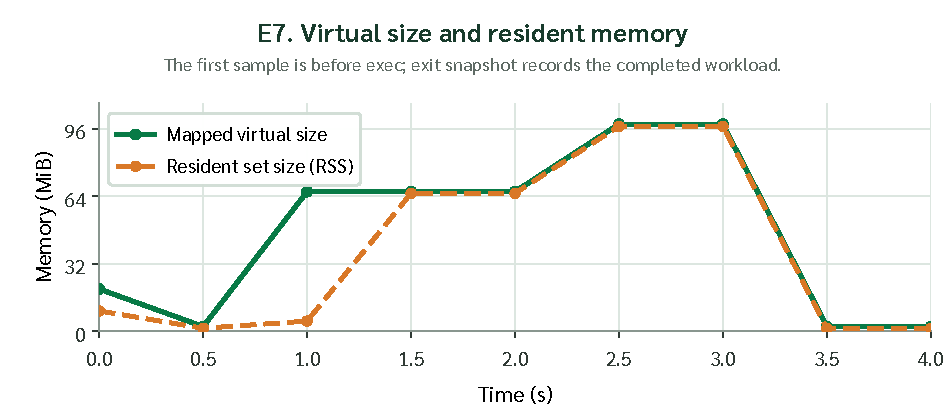
\includegraphics[width=\linewidth]{assets/timeline.pdf}
\caption{Virtual size and RSS recorded by the E7 command-line timeline}\end{figure}

When the program created an anonymous mapping, virtual size grew from about 2.2 MiB to 66.2 MiB before RSS reached the same level. At 1.0 second, RSS was 4.8 MiB. After the program touched the pages, RSS rose to 65.4 MiB. Mapping and reading a 32 MiB file increased the totals to about 98.2 MiB virtual size and 97.2 MiB RSS. After \code{munmap}, both returned close to their earlier levels. This run shows that reserving a range does not immediately make all of its pages resident in RAM.

The first watch-mode sample can occur between fork and exec or while the address space is changing. A sampled maximum should therefore not be treated as the child program's peak without checking the exit-time snapshot. The module reads the peak from the mm counters when the process exits. The reported minor/second and major/second rates use the counter difference divided by elapsed time between samples.

This is the terminal record used for the timeline figure and the values above. It includes the full sample sequence and exit-time totals.

\Needspace{34\baselineskip}
\lstinputlisting[basicstyle=\fontspec{Menlo}\fontsize{9}{11.5}\selectfont]{evidence/post-merge-5fbcb76/experiment-results/e7-timeline.txt}

\subsubsection{E8: process scope and descendants}

\begin{table}[H]\centering
{\fontsize{12}{15.6}\selectfont\arrayrulecolor{RuleGray}
\caption{E8 results under different fault scopes}
\begin{tabular}{|>{\raggedright\arraybackslash}p{6.0cm}|>{\raggedright\arraybackslash}p{2.4cm}|>{\raggedright\arraybackslash}p{2.2cm}|>{\raggedright\arraybackslash}p{3.8cm}|}
\hline
\rowcolor{SoftGreen} \textbf{Command} & \textbf{Minor} & \textbf{Major} & \textbf{Reference comparison} \\ \hline
\code{python3 -c pass} & 1,234 & 0 & Matches \code{getrusage()} \\ \hline
\code{sh + ls}, without \code{-f} & 258 & 0 & 135 below \code{wait4()} \\ \hline
\code{sh + ls}, with \code{-f} & 390 & 0 & Matches \code{wait4()} \\ \hline
\code{gcc}, without \code{-f} & 287 & 0 & 5,700 below \code{getrusage()} \\ \hline
\code{gcc}, with \code{-f} & 5,971 & 0 & Matches \code{wait4()} \\ \hline
\end{tabular}}
\end{table}

The shell and GCC launch other processes. In process-only mode, \code{pfstat} counts the selected process but not its children. The reference returned by \code{wait4()} can include usage from waited children. In these runs, enabling follow mode brought the \code{ls} and GCC results into agreement with their waited-descendant references. Python did not create a child and matched \code{getrusage()} in process-only mode. The differences in the table reflect the scope used by each counter; they do not by themselves show a counting error.

\code{wait4()} does not always include every descendant. A child may be auto-reaped when its parent sets \code{SIGCHLD} to \code{SIG\_IGN}. A child reparented before it is waited for may also be absent from the reference [4, 9]. The CLI therefore labels the reference as waited descendants only and explains when the live count exceeds it. The post-merge cleanup test covers the inherited \code{SIGCHLD=SIG\_IGN} case.

The saved E8 outputs make the scope difference visible for the same shell and compiler workloads:

\begin{lstlisting}
$ sudo tools/pfstat -- sh -c 'ls -R /usr/include >/dev/null'
  Minor faults 258; 135 below getrusage() because child usage is excluded
$ sudo tools/pfstat -f -- sh -c 'ls -R /usr/include >/dev/null'
  Minor faults 390; matches wait4() for waited descendants
$ sudo tools/pfstat -- gcc -O2 -o /tmp/fg tests/faultgen.c
  Minor faults 287; 5,700 below getrusage() because child usage is excluded
$ sudo tools/pfstat -f -- gcc -O2 -o /tmp/fg tests/faultgen.c
  Minor faults 5,971; matches wait4() for waited descendants
\end{lstlisting}

\Needspace{6\baselineskip}
\subsection{Step 3: Post-merge checks}

We reviewed and tested the source at merge commit \code{5fbcb767}; the measurements below come from that revision, not from a pre-merge branch. The original review focused on target changes during faults, PID reuse, concurrent thread exit, lifetime-counter aggregation, and session cleanup during module unload.

\begin{table}[H]\centering
{\fontsize{12}{15.6}\selectfont\arrayrulecolor{RuleGray}
\caption{Build, demo, and workflow checks after merge}
\begin{tabular}{|>{\raggedright\arraybackslash}p{2.8cm}|>{\raggedright\arraybackslash}p{5.8cm}|>{\raggedright\arraybackslash}p{5.9cm}|}
\hline
\rowcolor{SoftGreen} \textbf{Case} & \textbf{Check} & \textbf{Observed result} \\ \hline
Build and load & \code{make clean \&\& make all \&\& make load} & Passed; all proc entries were created \\ \hline
Demo & \code{make demo}; compare faults with \code{getrusage()} & Exit status 0; minor and major counts matched \\ \hline
Experiments & Run E1 to E8 with \code{scripts/experiments.sh} & Exit status 0; E8 scope differences were explained \\ \hline
Cleanup & Run \code{make clean} after testing & Passed; test binaries were removed \\ \hline
\end{tabular}}
\end{table}

The post-merge regression output is shown alongside these checks. It records the PID-reuse, concurrency, lifetime-counter, and unload cases completed by the suite.

\begin{figure}[H]\centering
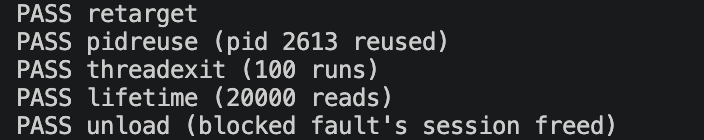
\includegraphics[width=.95\linewidth]{evidence/post-merge-5fbcb76/terminal/04-regression-terminal.png}
\caption{Terminal results from the post-merge lifecycle and concurrency regression suite.}
\end{figure}

\begin{table}[H]\centering
{\fontsize{12}{15.6}\selectfont\arrayrulecolor{RuleGray}
\caption{Lifecycle and concurrency regression checks after merge}
\begin{tabular}{|>{\raggedright\arraybackslash}p{2.8cm}|>{\raggedright\arraybackslash}p{5.8cm}|>{\raggedright\arraybackslash}p{5.9cm}|}
\hline
\rowcolor{SoftGreen} \textbf{Case} & \textbf{Check} & \textbf{Observed result} \\ \hline
Retarget & Generate faults in A, then select stopped process B & Passed; A's faults did not enter B's session \\ \hline
PID reuse & Reuse the numeric PID of an earlier target & Passed; old target remained exited and its counters did not change \\ \hline
Concurrent thread exit & End a thread group concurrently & Exit snapshots were complete in 100 runs \\ \hline
Lifetime aggregation & Read counters while creating and exiting threads & 20,000 reads; no counter decrease observed \\ \hline
Unload during a blocked fault & Unload while \code{userfaultfd} held a fault & Passed; canceled-probe sessions were released during unload \\ \hline
Inherited SIGCHLD & Run \code{pfstat -f -- /bin/true} with parent \code{SIGCHLD=SIG\_IGN} & Passed; child exited 0, target reset to idle, follow reset to N \\ \hline
\end{tabular}}
\end{table}

The merged source retains a reference to the session that accepted each fault until the return handler completes. It identifies targets by \code{struct pid}, uses \code{group\_dead} to detect the final thread, and protects lifetime totals with \code{stats\_lock}. It also releases sessions left by canceled probes during module unload [2]. In run mode, the program temporarily sets SIGCHLD to the default disposition while waiting and restores the child's inherited disposition before exec. The post-merge test confirmed that \code{wait4()} still collects the child status and that cleanup returns the target and follow state to idle and N.

The source sets \code{0600} on \code{/proc/pfcount/target} and \code{0400} on \code{stats} and \code{maps}. A non-root permission check appears in the pre-merge evidence, but we did not rerun that case after merge, so it is not listed as a post-merge regression result.

The inherited SIGCHLD cleanup check also captured the process summary and the final idle state of the module:

\lstinputlisting{evidence/post-merge-5fbcb76/04-sigchld-cleanup.txt}

GitHub Actions checks were not configured for the branch we reviewed. The build and regression results in this report came from manual runs inside Lima, not from an automated GitHub workflow [10].

\Needspace{6\baselineskip}
\section{Problem 3: Limitations and conclusion}

\subsection{Step 1: Limitations}

The results apply to Ubuntu 24.04.5, Linux 6.8.0-142-generic, ARM64, and the kernel options in Table 2. Without \code{CONFIG\_BSD\_PROCESS\_ACCT=y}, the module cannot register the \code{acct\_collect()} probe and therefore cannot capture exit snapshots. It can still report a running target, but it cannot confirm final values for a short-lived process [2]. VMA iteration and probe arguments also depend on kernel APIs, so other versions and architectures need separate builds and checks.

Live counters begin when a target is selected. Descendant tracking follows \code{real\_parent} ancestry up to 64 levels, and reparenting can change which processes are in scope. \code{wait4()} reports usage passed through waited children; auto-reaped or reparented children may be absent. Comparisons must use the same time window and process scope.

The kretprobe runs on the page-fault path before filtering the target and uses \code{maxactive=64}. If more concurrent invocations occur than the probe can handle, the kernel increments \code{nmissed} [8]. The recorded runs showed no reported probe misses, but we did not measure overhead under sustained fault load. A follow-up measurement should compare the same workload with the module unloaded, loaded without a target, and loaded with a target.

The module, maps, status, and stat interfaces are read at different times. A process that changes mappings or creates threads during a comparison can produce differences due to timing. Stable or paused targets make structural comparisons easier to interpret. The report also retains byte-level values before converting them to rounded display units.

Results from E3 to E6 depend on page-cache state, readahead, fault-around, and whether the kernel accepts the THP advice. \code{POSIX\_FADV\_DONTNEED} and \code{MADV\_HUGEPAGE} do not guarantee a fixed outcome. We did not collect \code{AnonHugePages} for every mapping, so the THP result is suggestive rather than proof that all pages were backed by huge pages.

The comparisons with \code{/proc/PID/stat}, \code{getrusage()}, and \code{wait4()} are consistency checks against counters maintained by the same Linux kernel. They are not independent external measurements. The tests did not cover another kernel version, x86\_64, another PID namespace, or a systematic performance benchmark.

\Needspace{6\baselineskip}
\subsection{Step 2: Conclusion}

The tool accepts a PID and reports the four values required by the assignment. After merge, the region count and virtual size matched procfs for the recorded targets, and the page-fault counters matched kernel references when the process scope and time window aligned. E2 to E7 also showed that virtual size can grow before RSS and that page-cache state, readahead, fault-around, and THP requests affect observed fault counts.

The build, demo, regression suite, and experiments E1 to E8 passed in the documented Lima environment. These results support the implementation for the tested workloads and configuration. They do not establish compatibility with every Linux kernel or architecture, and the probe overhead remains unmeasured.

\clearpage
\Needspace{6\baselineskip}
\section*{References}\addcontentsline{toc}{section}{References}

[1] CPE333 Mini-Project 2 assignment, Academic Year 2026, pp. 2-5.\\
{\fontsize{12}{15.6}\selectfont\url{../CPE333_MiniProject2_2026.pdf}}\par

[2] beambeambeam/cpe333, Mini-Project 02 source after PR \#11 was merged.\\
{\fontsize{12}{15.6}\selectfont\url{https://github.com/beambeambeam/cpe333/tree/5fbcb7679298f36e2bae8b7cd3dbe6bf6a609800/mini-project-02}}\par

[3] The Linux Kernel documentation, Process Addresses.\\
{\fontsize{12}{15.6}\selectfont\url{https://docs.kernel.org/mm/process_addrs.html}}\par

[4] Linux man-pages, \code{getrusage(2)}, resource usage and child accounting.\\
{\fontsize{12}{15.6}\selectfont\url{https://man7.org/linux/man-pages/man2/getrusage.2.html}}\par

[5] Linux v6.8 source, \code{mm/memory.c}: \code{handle\_mm\_fault()} and \code{mm\_account\_fault()}.\\
{\fontsize{12}{15.6}\selectfont\url{https://github.com/torvalds/linux/blob/v6.8/mm/memory.c}}\par

[6] Linux man-pages, \code{madvise(2)}, mapping and huge-page advice.\\
{\fontsize{12}{15.6}\selectfont\url{https://man7.org/linux/man-pages/man2/madvise.2.html}}\par

[7] Linux v6.8 source, \code{fs/proc/array.c}: \code{do\_task\_stat()} and \code{stats\_lock}.\\
{\fontsize{12}{15.6}\selectfont\url{https://github.com/torvalds/linux/blob/v6.8/fs/proc/array.c}}\par

[8] The Linux Kernel documentation, Kernel Probes.\\
{\fontsize{12}{15.6}\selectfont\url{https://docs.kernel.org/trace/kprobes.html}}\par

[9] Linux v6.8 source, \code{kernel/exit.c}: \code{do\_exit()}, \code{group\_dead}, and waited-child accounting.\\
{\fontsize{12}{15.6}\selectfont\url{https://github.com/torvalds/linux/blob/v6.8/kernel/exit.c}}\par

[10] PR \#11 review discussion and revisions.\\
{\fontsize{12}{15.6}\selectfont\url{https://github.com/beambeambeam/cpe333/pull/11}}\par

\clearpage
\Needspace{6\baselineskip}
\section*{Appendix: Reproduction steps and evidence}\addcontentsline{toc}{section}{Appendix: Reproduction steps and evidence}

The report uses the merged source at commit \code{5fbcb767}. The source code and its build, experiment, and regression scripts are in the team's \href{https://github.com/beambeambeam/cpe333/tree/5fbcb7679298f36e2bae8b7cd3dbe6bf6a609800/mini-project-02}{Mini-Project 2 source folder}. The steps below reproduce the recorded Linux run from a macOS host with Homebrew and Lima.

\begingroup
\setlength{\parskip}{2.5pt}
\titlespacing*{\subsection}{0pt}{5pt}{1pt}
\lstset{basicstyle=\fontspec{Menlo}\fontsize{9}{10.5}\selectfont,aboveskip=3pt,belowskip=3pt}

\subsection{Step 1: Check out the tested source}

Clone the team repository and select the exact merge commit used for the report. This keeps later changes on \code{main} from changing the source under test.

\begin{lstlisting}[language=sh]
git clone https://github.com/beambeambeam/cpe333.git
cd cpe333/mini-project-02
git checkout 5fbcb7679298f36e2bae8b7cd3dbe6bf6a609800
\end{lstlisting}

\subsection{Step 2: Create and prepare the Lima VM}

Run the project helper from the \code{mini-project-02/} directory. If Lima is not installed, the helper installs it with Homebrew. It creates an Ubuntu 24.04 VM, mounts the project directory read-write, and installs the compiler, Python, and headers for the guest kernel.

\begin{lstlisting}[language=sh]
./vm.sh setup
./vm.sh run uname -a
\end{lstlisting}

The tested guest used Ubuntu 24.04.5, Linux 6.8.0-142-generic, and ARM64. The module needs \code{CONFIG\_KPROBES=y}, \code{CONFIG\_KRETPROBES=y}, and \code{CONFIG\_BSD\_PROCESS\_ACCT=y}; the recorded values are in \code{evidence/post-merge-5fbcb76/00-environment.txt}.

\subsection{Step 3: Build and load the module}

Run these commands from the source directory on the macOS host. The helper executes each Make target inside the VM. \code{make all} builds the module and the \code{faultgen} test program; \code{make load} inserts the module and checks that its proc entries exist.

\begin{lstlisting}[language=sh]
./vm.sh make clean
./vm.sh make all
./vm.sh make load
./vm.sh run ls -l /proc/pfcount
\end{lstlisting}

The module exposes three interfaces under \code{/proc/pfcount}:

\begin{lstlisting}[language=sh]
/proc/pfcount/target
/proc/pfcount/stats
/proc/pfcount/maps
\end{lstlisting}

The recorded build skipped BTF because \code{vmlinux} was unavailable; compilation and module loading still completed.

\Needspace{14\baselineskip}
\subsection{Step 4: Inspect a live process}

Open a VM shell, start a stable process, then compare \code{pfstat --maps} with \code{/proc/PID/maps}.

\begin{lstlisting}[language=sh]
./vm.sh shell
sleep 300 &
PID=$!
sudo tools/pfstat "$PID" --maps
sudo cat /proc/"$PID"/maps
kill "$PID"
exit
\end{lstlisting}

Check that the VMA count and summed ranges match \code{/proc/PID/maps}; compare virtual size with \code{VmSize} and lifetime faults with \code{/proc/PID/stat}.

\subsection{Step 5: Run the demo and regression checks}

The demo watches \code{faultgen}, then compares exit-time counts with \code{getrusage()}. The regression suite covers retargeting, PID reuse, thread exit, lifetime-counter reads, and unload during a blocked fault.

\begin{lstlisting}[language=sh]
./vm.sh make demo
./vm.sh run sudo sh tests/regress.sh
\end{lstlisting}

The latest demo transcript and regression log are in \path{evidence/post-merge-5fbcb76/02-demo-terminal-capture.txt} and \path{evidence/post-merge-5fbcb76/03-regression.txt}; the demo screenshot is a separate, labeled run.

\subsection{Step 6: Run experiments E1 to E8}

The script rebuilds helpers, reloads the module, runs the procfs comparison and controlled workloads, records output in \code{results/}, then unloads the module.

\begin{lstlisting}[language=sh]
./vm.sh make experiments
\end{lstlisting}

E1 cross-checks procfs; E2 to E6 vary mapping type, cache state, readahead, and THP advice; E7 samples virtual size and RSS while the workload maps and frees memory; E8 compares process-only with descendant tracking. The report explains each result, and raw outputs are in \code{evidence/post-merge-5fbcb76/experiment-results/}.

\subsection{Step 7: Unload and remove build artifacts}

Unload the module, remove generated binaries, and stop Lima. These commands preserve the source and saved evidence.

\begin{lstlisting}[language=sh]
./vm.sh make unload
./vm.sh make clean
./vm.sh stop
\end{lstlisting}

The evidence bundle contains environment, build/load, demo, regression, cleanup, and E1 to E8 records, plus six Terminal captures. Full output remains in searchable text files.

\endgroup
\end{document}
